\section{Durchführung}
\label{sec:Durchführung}

Die Versuchsaufbau erfolgt gemäß \autoref{fig:aufbau}.
\begin{figure}[H]
	\centering
	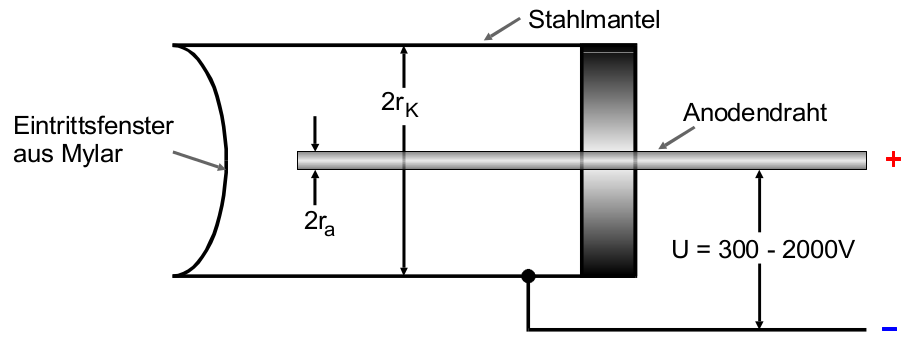
\includegraphics[width=0.8\textwidth]{content/aufbau.png}
	\caption{Skizze der Messapparatur \cite{sample}}
	\label{fig:aufbau}
\end{figure}

\noindent
Als Quelle dient hier ein $^{204}\text{Tl}$-Präparat, welches für die Vermeidung von Totzeitkorrekturen so platziert 
wurde, dass bei mittlerer Zählrohrspannung die Zählrate kleiner als $100$ Imp/s war. Dazu soll $U$ unter $\SI{700}{\volt}$
bleiben, da sonst der Bereich der Selbstentladung erreicht wird, wo das Zählrohr zerstört wird.

\subsection{Aufnahme der Charakteristik und des Zählrohrstroms}
\label{sec:durch:charakteristik}

Für die Aufnahme der Charakteristik wird gemäß \autoref{sec:theo:charakteristik} das Zählrohr mit konstanter 
Intensität bestrahlt. Die Spannung wird in Schritten von $\Delta U = \SI{10}{\volt}$ variiert. Da der Plateuanstieg
sehr gering ist, müssen die Werte für die Spannung sehr genau gemessen werden; der relative statistische Fehler soll
kleiner als $1\%$ sein. Da die Zählraten Poisson verteilt sind, liegt die Messunsicherheit bei $\Delta N = \sqrt{N}$.
Für die Präzisionsanforderung muss $N$ von der Größenordnung $10000$ Imp/s sein.
\begin{equation}
	\frac{\Delta N}{N} = \frac{\sqrt{N}}{N} = \frac{1}{\sqrt{N}} \overset{!}{\leq} 0.01 
	\Rightarrow N \geq 100^2 = 10000
\end{equation}
\noindent
Bei der gewählten Quelle entspricht das einer Integrationszeit pro Zählrohrspannung von $t = \SI{60}{\second}$.
\\
Zusätzlich zu den Zählraten wird alle $\SI{50}{\volt}$ der Zählrohrstrom $I$ abgelesen und notiert.

\subsection{Sichtbarmachung von Nachentladungen}
\label{sec:duch:nachentladungen}

Für diesen Versuchsteil wird die Spannung zunächst auf ungefähr $\SI{350}{\volt}$ abgesenkt. 
Die Intensität der Strahlungsquelle wird ebenfalls herabgesenkt, sodass auf dem Oszillographen 
nur ein Ladungsimpuls pro Durchlauf zu sehen ist. Danach wird die Röhrenspannung stark erhöht (unter Beachtung dass
keine Selbstentladungen ausgelöst werden). Nun sollten Nachentladungen sichtbar sein, die zweitliche Differenz 
zwischen Primär- und Nachentladungimpuls soll dabei gemessen werden.

\subsection{Oszillographische Messung der Totzeit}
\label{sec:durch:oszill-totzeit}

Wie in \autoref{sec:theo:oszillographisch} beschrieben, muss eine hohe Strahlungsintensität eingestellt werden und der
Trigger auf die Anstiegsflanke gestellt werden. Bei einem Oszillogramm, welches dem aus \autoref{fig:totzeit} ähnelt,
kann eine Momentaufnahme gemacht werden, wobei die Skalierung der Zeitachse mit notiert werden muss.

\subsection{Totzeitbestimmung mit der Zwei-Quellen-Methode}
\label{sec:durch:zwei-quellen}

Für diesen Versuchsteil wird die Strahlungsquelle näher an das Zählrohr bewegt, um Totzeitkorrekturen zu erhalten. Danach
erfolgt Vorgehen gemäß \autoref{sec:theo:zwei-quellen}, d.h. die Zählraten für die Quellen einzeln ($N_1$ und $N_2$)
und beide Quellen zusammen ($N_{1+2}$) über einen Zeitraum hinweg messen.
